\documentclass[12pt,spanish]{article}
\usepackage[spanish]{babel}
\usepackage{graphicx}
\usepackage{color}
\usepackage{colortbl}
\usepackage{amsthm,thmtools}
\usepackage{dirtytalk}
\usepackage{multirow}
\usepackage{amsmath}
\usepackage{subcaption}
\usepackage{adjustbox}
\usepackage{amsmath}
\usepackage{centernot}
\usepackage{mathtools}
\usepackage{multirow}
\usepackage[hidelinks]{hyperref}
\usepackage{caption}
\usepackage{eurosym} % para el euro
\usepackage{amsthm}
\usepackage{multicol}
\usepackage{float}
\usepackage{amsfonts}
\usepackage{titling}
\usepackage{soul}
\usepackage{listings}
\usepackage{array}
\usepackage{tikz}
\usepackage{apacite}
\usepackage{etoolbox}
\usepackage{xcolor}
\usetikzlibrary{shapes.geometric, arrows, chains, calc,positioning,fit,decorations.pathreplacing}
\usepackage[framemethod=tikz]{mdframed}

\graphicspath{ {../img/}}
\selectlanguage{spanish}
\usepackage[utf8]{inputenc}
\usepackage{graphicx}
\usepackage[a4paper,left=3cm,right=2cm,top=2.5cm,bottom=2.5cm]{geometry}

\lstset{
  breaklines=true,
  postbreak=\mbox{\textcolor{red}{$\hookrightarrow$}\space},
}

\newcommand{\quotebox}[1]{\begin{center}\fcolorbox{white}{blue!10}{\begin{minipage}{0.9\linewidth}\vspace{10pt}\center\begin{minipage}{0.8\linewidth}{\space\Huge``}{#1}{\hspace{1.5em}\break\null\Huge\hfill''}\end{minipage}\smallbreak\end{minipage}}\end{center}}

\title{Computación Ubicua e Inteligencia Ambiental}
\setlength{\droptitle}{10em}
\author{Carlos Sánchez Páez}

\makeindex
\begin{document}
\definecolor{light-gray}{gray}{0.95}
\lstset{columns=fullflexible,basicstyle=\ttfamily}
\surroundwithmdframed[
  hidealllines=true,
  backgroundcolor=light-gray,
  innerleftmargin=0pt,
  innertopmargin=0pt,
  innerbottommargin=0pt]{lstlisting}


\begin{titlepage}

 \newlength{\centeroffset}
 \setlength{\centeroffset}{-0.5\oddsidemargin}
 \addtolength{\centeroffset}{0.5\evensidemargin}
 \thispagestyle{empty}

 \noindent\hspace*{\centeroffset}
 \begin{minipage}{\textwidth}

  \centering
  
\includegraphics[width=0.9\textwidth]{logo_ugr.jpg}\\[1.4cm]

  \textsc{ \Large Computación Ubicua e Inteligencia Ambiental\\[0.2cm]}
  \textsc{GRADO EN INGENIERÍA INFORMÁTICA}\\[1cm]

  {\Huge\bfseries ARWrite \\}
 \end{minipage}

 \vspace{1.5cm}
 \noindent\hspace*{\centeroffset}
 \begin{minipage}{\textwidth}
  \centering

  \textbf{Autor}\\ {Carlos Sánchez Páez}\\[2.5ex]
  
\includegraphics[width=0.4\textwidth]{etsiit_logo.png}\\[0.1cm]
  \vspace{1.5cm}
  
\includegraphics[width=0.15\textwidth]{decsai.jpg}\\[0.1cm]
  \vspace{1cm}
  \textsc{Escuela Técnica Superior de Ingenierías Informática y de Telecomunicación}\\
  \vspace{1cm}
  \textsc{Curso 2019-2020}
 \end{minipage}
\end{titlepage}
\thispagestyle{empty}
\newpage
\tableofcontents{}
\newpage

\section{Descripción de la app}

El objetivo de este proyecto es desarrollar una aplicación basada en realidad aumentada que se utilizará para reforzar la enseñanza del trazo y la caligrafía a niños/as de infantil. Ésto se conseguirá haciendo que el usuario (niño/a) intente dibujar una letra (elegida por el profesor/a) en el aire con un puntero. El sistema identificará mediante técnicas de OCR la entrada e informará si coincide con lo esperado.\\

La aplicación constará de dos ventanas, una en la que se verá la letra objetivo y otra que mostrará la captura de video y el trazo dibujado hasta el momento.\\

\begin{figure}[H]
	\centering
	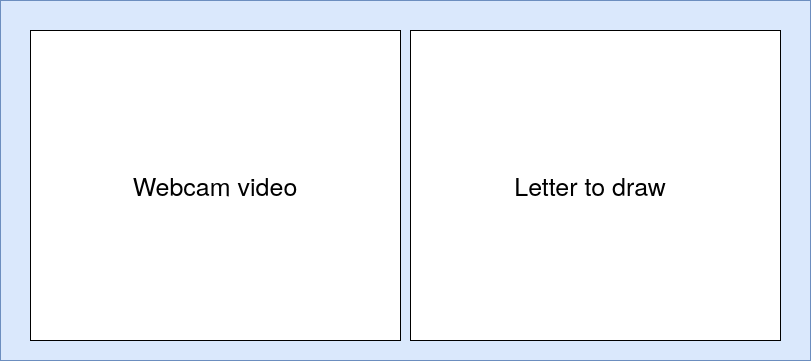
\includegraphics[scale=0.5]{initial_app_layout.png}
	\caption{Diseño de la aplicación}
\end{figure}

\newpage
\section{Motivación}

\subsection{Problema a resolver}
\label{problema}

La tecnología tiene un rol clave hoy día en prácticamente todos los ámbitos de nuestra vida. En el educativo, las clases cada vez se enriquecen más gracias a recursos digitales. Esto ocurre en prácticamente todos los sectores, desde el infantil hasta las altas titulaciones. \\

En el caso de las primeras etapas escolares de los alumnos (infantil), la enseñanza apoyada por medios digitales se hace cada vez más necesaria. En \cite{Robles-Melendez} se justifica su uso en el aula ya que potencian la motivación y comprensión de la materia para el alumno. Podemos contrastar la efectividad de las mismas en publicaciones como \cite{Bonneton-Botte2020}, que propone una aplicación para aprender a escribir en una tablet.\\

En este proyecto se pretende aprovechar la serie de ventajas que trae la tecnología al aula para conseguir que el alumno/a desarrolle el aprendizaje del trazo de una forma motivadora y amena, cambiando la tradicional escritura en pizarra por escritura en realidad aumentada.

\subsection{Competencia}

En la actualidad ya existen aplicaciones de realidad aumentada orientada a la educación de preescolar. Por ejemplo, QuiverVision \cite{quiver} ofrece una aplicación en la que el usuario colorea unas plantillas con dibujos y al enfocarlas con una tablet o smartphone, el dibujo se vuelve interactivo, ofreciendo al alumno/a jugar con el personaje que ha dibujado. Math Alive \cite{MathAlive} propone juegos que consisten en colocar cartas frente a una cámara para aprender a contar y realizar operaciones básicas.\\

Existen más aplicaciones de realidad aumentada enfocadas a la educación en preescolar, pero se centran en que el alumno/a rellene fichas y las enfoque con la cámara para hacerlas interactivas o bien. Aquí se encuentra el elemento diferenciador del proyecto: el usuario realizará el trazo frente a la pantalla y la aplicación le proporcionará un \emph{feedback}.

\begin{figure}[H]
	\centering
	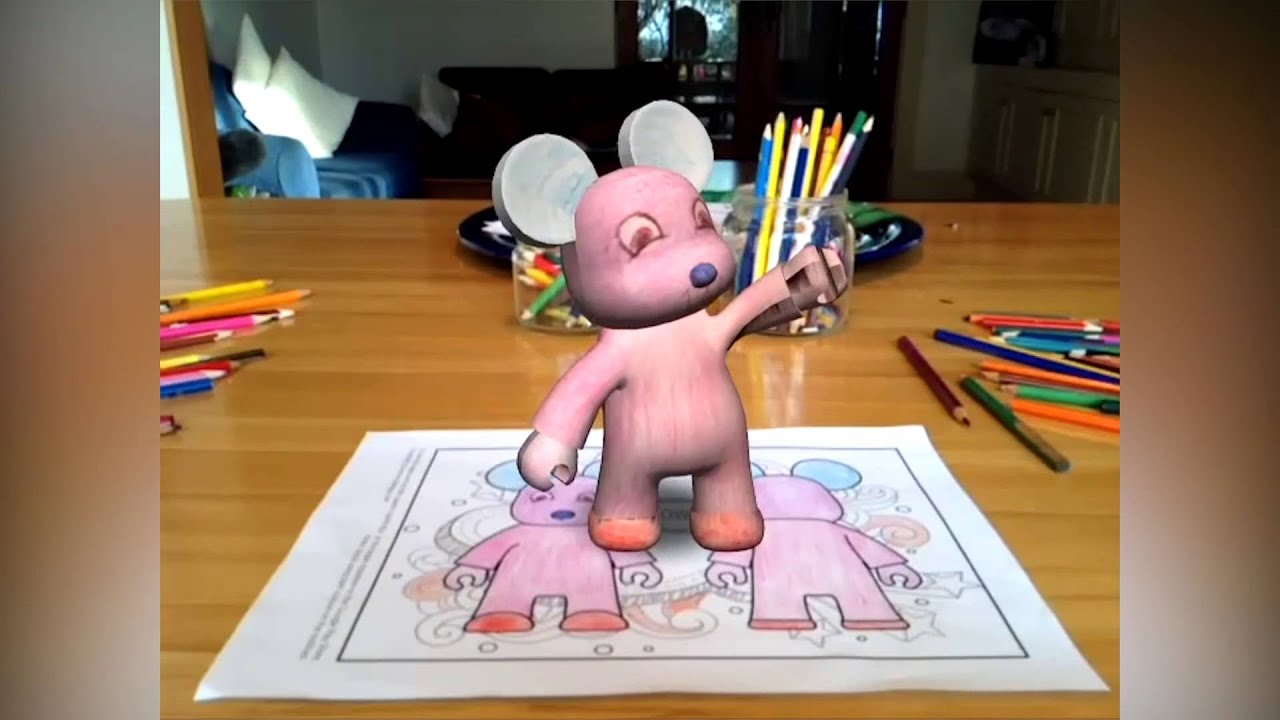
\includegraphics[scale=0.2]{quiver.jpg}
	\caption{\emph{Quiver} en funcionamiento}
\end{figure}

\subsection{Opiniones de expertos}

En la sección \ref{problema} podemos consultar varias referencias bibliográficas que avalan la efectividad de las aplicaciones de realidad aumentada en el ámbito escolar. Además, contamos con la opinión de Isabel María Páez Alba, diplomada en Educación General Básica en la especialidad de filología francesa por la Escuela Universitaria María Inmaculada de Antequera (Málaga) en el año 1988 y que lleva ejerciendo como profesora de educación infantil durante 31 años:

\quotebox{
\footnotesize
  La Ley Orgánica 2/2006, de 3 de mayo, de Educación y el Decreto 428/2008, de 29 de julio, establecen la ordenación y las enseñanzas correspondientes a la Educación Infantil en Andalucía. La Educación Infantil es concebida como una etapa única en la que se inicia a los niños y niñas de 3, 4 y 5 años en determinados aprendizajes. Por ello, en esta etapa, la ley propone un acercamiento a la lectoescritura. La escritura sigue siendo un aprendizaje básico para toda persona. Es la forma en la que podemos comunicarnos, expresar nuestros sentimientos, intercambiar opiniones; en definitiva, es la forma en la que podemos trasmitir. Es en esta etapa donde  van a tener su primer contacto con el lenguaje escrito;  es un reto arduo al que los niños y niñas se enfrentan. Antes de escribir es necesario que el niño domine y controle sus movimientos, que sea capaz de desplazar la mano en el sentido deseado; debe adquirir habilidad grafomotriz. Todo esto se adquiere de forma lúdica y activa, principios metodólogicos básicos y fundamentales en la Educación Infantil.\\\\
  El proyecto presentado por D. Carlos Sánchez Páez aúna cuatro aspectos relevantes en el aprendizaje lectoescritor. Por un lado, va a iniciar al niño/a en el proceso de la escritura. Por otro, va a dotar al alumnado de un soporte motivador, innovador, atractivo para los niños y niñas. Las nuevas tecnologías son tremendamente atractivas para esta generación de alumnos que han nacido en esta era.  En tercer lugar, va a favorecer la autocorrección y autoevaluación. El niño/a va  a ser artífice de su propio aprendizaje. Y por último y no por eso  menos importante, ofrece a los niños y niñas los principios metodológicos fundamentales para el aprendizaje en su corta edad: actividad y juego. En definitiva, se aglutina en este proyecto toda la base de una enseñanza completa, atractiva, divertida y personalizada.
}
\newpage
\section{Recursos a utilizar}

Para el desarrollo del proyecto se pretenden utilizar las siguientes tecnologías:
\begin{itemize}
	\item \textbf{Plataforma destino}: PC
	\item \textbf{Lenguaje de programación}: Python \cite{python}
	\item \textbf{Frameworks}
		\begin{itemize}
			\item OpenCV \cite{opencv}. Librería orientada a la visión por computador en tiempo real.
			\item Keras \cite{Keras}. Librería orientada a redes neuronales. Se utilizará junto a MNIST \cite{mnist}, una base de datos de dígitos escritos a mano para construir una red neuronal que clasificará la entrada del usuario.
		\end{itemize}
\end{itemize}

\section{Descripción detallada de la aplicación}

La aplicación seguirá el siguiente esquema:
\begin{enumerate}
  \item La aplicación muestra un cuadro de dialogo solicitando una letra objetivo.
  \item El usuario elige la letra objetivo.
  \item La ventana principal de la aplicación se abre. En el lado izquierdo se ve la captura de la cámara y en el derecho la letra elegida por el usuario en fuente escolar.
  \item El usuario toma su marcador y dibuja la letra en el aire. Cuando termine, deberá ocultar la parte azul del marcador a la cámara.
  \item La aplicación procesa el trazo y lo envía a la red neuronal previamente entrenada para obtener una predicción.
  \item Si la predicción es correcta, se le preguntará al usuario si desea jugar otra vez. En caso contrario, se informará de la letra que ha dibujado y se le pedirá que lo intente de nuevo.
\end{enumerate}

En esta aplicación se ha implementado el uso de un marcador de color azul, como por ejemplo un rotulador de pizarra con el tapón puesto. El resto del cuerpo del marcador deberá ser de otro color para que al girarlo se oculte.

\begin{figure}[H]
	\centering
	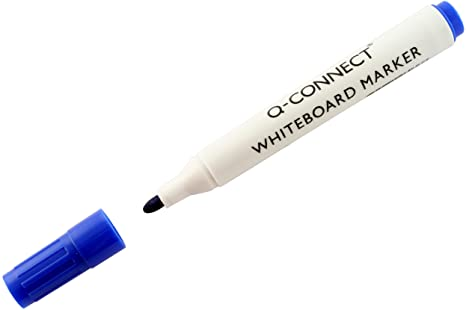
\includegraphics[width=0.5\textwidth]{rotulador.jpg}
	\caption{Ejemplo de marcador válido}
\end{figure}

Junto a la aplicación en sí, se adjunta un ejecutable para distribuciones Linux que instala la aplicación y sus dependencias además de crear las correspondientes entradas en el menú de aplicaciones (aplicación y desinstalador).
\begin{figure}[H]
	\centering
	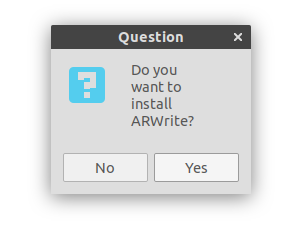
\includegraphics[width=0.5\textwidth]{installer.png}
	\caption{Instalador de ARWrite}
\end{figure}
\begin{figure}[H]
	\centering
	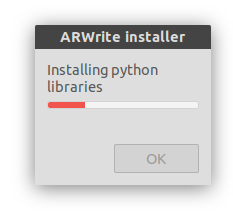
\includegraphics[width=0.5\textwidth]{installer2.png}
	\caption{Instalador de ARWrite (2)}
\end{figure}
\begin{figure}[H]
	\centering
	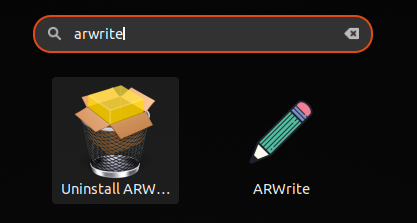
\includegraphics[width=0.5\textwidth]{entries.png}
	\caption{Entradas en el menú de aplicaciones}
\end{figure}

\begin{figure}[H]
	\centering
	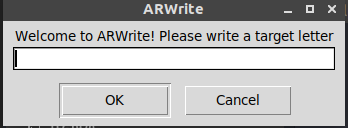
\includegraphics[width=0.5\textwidth]{inputletter.png}
	\caption{Solicitud de letra objetivo}
\end{figure}
\begin{figure}[H]
	\centering
	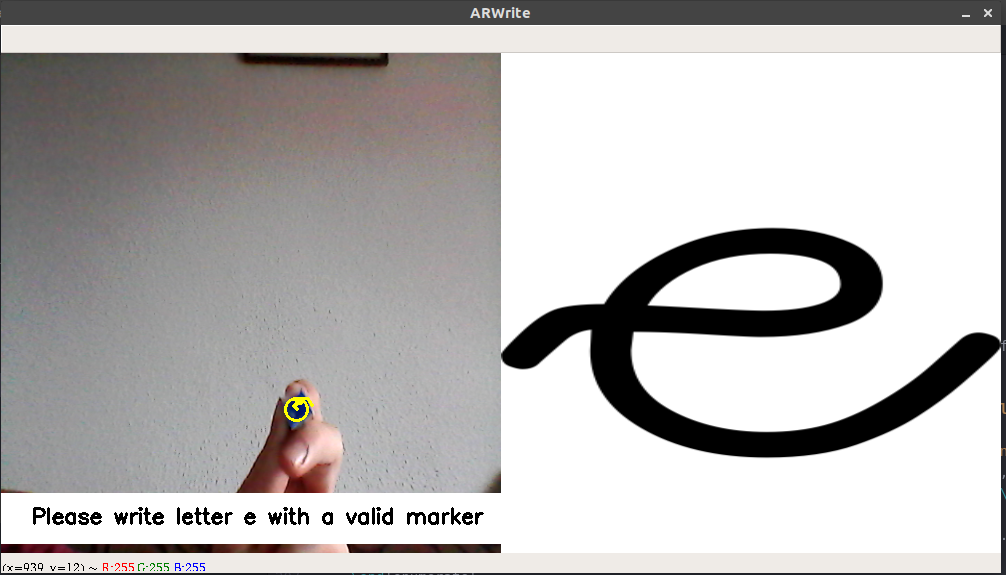
\includegraphics[width=0.75\textwidth]{app1.png}
	\caption{Ventana principal de la app}
\end{figure}

\begin{figure}[H]
	\centering
	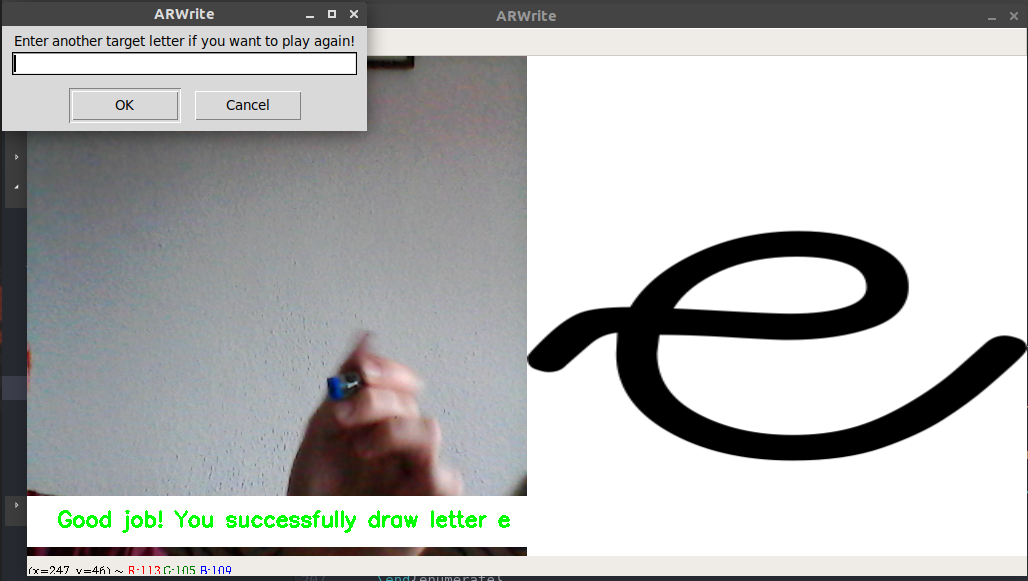
\includegraphics[width=0.75\textwidth]{letter_ok.png}
	\caption{Letra dibujada correctamente}
\end{figure}

\begin{figure}[H]
	\centering
	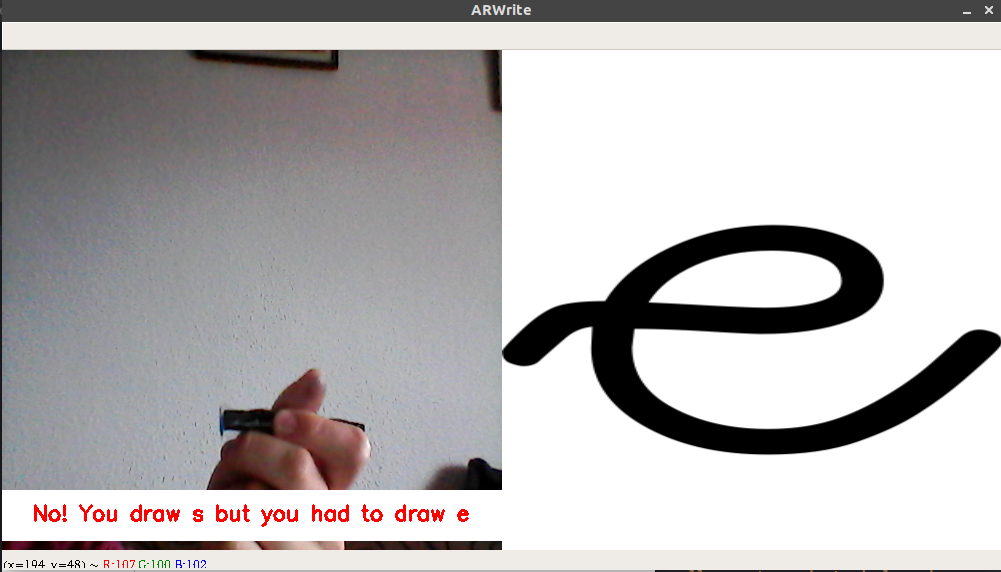
\includegraphics[width=0.75\textwidth]{wrong_letter.png}
	\caption{Letra incorrecta dibujada}
\end{figure}

\section{Aprendizaje del entorno}

Durante el diseño y la implementación de la aplicación los entornos utilizados fueron los siguientes:
\begin{enumerate}
  \item \textbf{Frameworks para el desarrollo y entrenamiento de la red neuronal}
  \begin{enumerate}
    \item Keras \cite{Keras}. Es una librería escrita sobre TensorFlow \cite{tensorflow} que permite la implementación a alto nivel de redes neuronales. En la apliacción se utilizarán redes neuronales de tipo convolucional, con las que ya he trabajado antes (\url{https://github.com/csp98/image-recognition})
    \item Numpy \cite{numpy}. Biblioteca para procesamiento científico de datos. Es necesaria para trabajar con varias dimensiones en el desarrollo de la red neuronal.
  \end{enumerate}
  \item \textbf{Framework para realidad aumentada}: OpenCV \cite{opencv}. Usada para capturar la imagen desde la cámara, identificar el marcador, dibujar los trazos en la pantalla, etc. Es la piedra angular de la aplicación.
  \item \textbf{Frameworks para manejar interfaces gráficas}
    \begin{enumerate}
      \item Tkinter \cite{tkinter}. Biblioteca de Python \cite{python} que utiliza para mostrar la ventana en la que se solicita la letra objetivo al usuario.
      \item Zenity \cite{zenity}. Aplicación de Linux que se usa para crear la interfaz gráfica del instalador y desinstalador.
      \item Pkexec \cite{pkexec}. Utilidad gráfica de Linux para solicitar permisos de superusuario. Se usa en el instalador.
    \end{enumerate}

\end{enumerate}



\newpage
\bibliographystyle{apacite}
\bibliography{refs}

\end{document}
